\documentclass[11pt, a4paper]{article}
\usepackage[utf8]{inputenc}
\usepackage{graphicx}
\usepackage{booktabs} % For \toprule, \midrule and \bottomrule
\usepackage{pgfplotstable} % Generates table from .csv

% change default font family from serif to sans-serif
\renewcommand{\familydefault}{\sfdefault}

\title{IHK-Projektantrag}
\date{2019-03-25}
\author{John Doe}

\begin{document}

\maketitle
\noindent{Beruf\quad \quad \quad Fachinformatiker Anwendungsentwicklung}\newline
Pr{\"u}fung\quad \quad 0\newline

\section{Projektbezeichnung}
Entwicklung einer Customer REST-API mit Web-Interface

\section{Aufgabenstellung}
Die Projektaufgabe besteht darin eine REST API Web Application zu entwickeln,
mit welcher Kunden-Datensaetze einem unternehmensinternen Datenbankserver durch
autorisierte Benutzer hinzugefuegt, abgerufen, aktualisiert und geloescht werden
koennen. Zusaetzlich soll zur einfacheren Bedienung durch Mitarbeiter ein auf
HTML5 basierendes grafisches Web-Interface erstellt werden.

\section{Projektziele}
Am Ende des Projektes soll eine voll-funktionsfähige Express.js Web App, ein
MongoDB Datenbank Server, ein React.js Web-Interface, und die dazugehörige
Softwaredokumentation geliefert werden.

Die Web App ist eine REST API, welche die nötigen HTTP Routen, das Datenmodel
und eine Input-Validierung aufweisen muss. Das zu erstellende Datenbankmodel
muss in MongoDB kompatiblem Code umgewandelt werden und durch das
Produktionsteam leicht in den bestehenden Datenbankserver zu integrieren sein.
Konfiguration der Web-App und der Datenbank soll leicht über Umgebungsvariablen
und/oder im Projekt enthaltene Konfigurationsdateien erfolgen.

Benutzer werden mit JSON-Web-Tokens authentifiziert und autorisiert.
Kundenpasswoerter werden mit bcrypt gehasht bevor sie in der Datenbank
gespeichert werden. Das Produktionsteam wird darauf hingewiesen, dass der
zentrale Datenbankserver ausreichend gesichert sein muss.

Das Web-Interface muss über einen Webserver hostbar sein, und die wichtigen
Funktionen der REST API in grafischer Form präsentieren.

Das Kostenziel für das gesamte Projekt beträgt 200 Euro.

Das Terminziel des Projektes ist der 12.04.2019, 12:30 Uhr.

\section{Projektstrukturplan}
Ein Projektstrukturplan in Diagramform ist erstellt und im Anhang ersichtlich.

\subsection{Hauptaufgaben auflisten}
\begin{itemize}
  \item Definitionsphase
  \item Planungsphase
  \item Implementierungsphase
  \item Abschlussphase
\end{itemize}

\subsection{Teilaufgaben (mit Zeitrahmen) auflisten}
Der Projektstrukturplan ist um die Anzahl Stunden pro Arbeitspaket erweitert,
als Terminplan im Tabellenformat im Anhang ersichtlich.



\noindent A. Definitionsphase (8h)
\begin{enumerate}
  \item Situationsanalyse (2h)
  \item Auftragsbeschreibung (1h)
  \item Problemdefinition (1h)
  \item Fragenkatalog erstellen (1h)
  \item Kundengespräch (1h)
  \item Ist-Analyse (1h)
  \item Soll-Konzept (1h)
\end{enumerate}

\noindent B. Planungsphase (12h)
\begin{enumerate}
  \item Projektstrukturplan erstellen (1h)
  \item Zeitplan erstellen (1h)
  \item Kostenplan erstellen (1h)
  \item Qualitätssicherungsplan erstellen (1h)
  \item Use Case Diagramm erstellen (2h)
  \item Klassendiagramme erstellen (4h)
  \item Datenbankmodel erstellen (2h)
\end{enumerate}

\noindent C. Implementierungsphase (40h)
\begin{enumerate}
  \item Unit Tests schreiben (4h)
  \item REST-API Code entwickeln (8h)
  \item Datenbank-Code entwickeln (8h)
  \item Web-Interface entwickeln (8h)
  \item Datenbank, API und Interface integrieren (8h)
  \item Systemtests durchführen (4h)
\end{enumerate}

\noindent D. Abschlussphase (10h)
\begin{enumerate}
  \item Soll-Ist Vergleich durchführen (1h)
  \item Projektdokumentation fertigstellen (7h)
  \item Projektübergabe (1h)
  \item Fazit (1h)
\end{enumerate}

Gesamt: 70 Stunden

\section{Pr{\"a}sentation}
\subsection{Geplante Pr{\"a}sentationsmittel}
Fuer die Praesentation wird ein Beamer und Laptop benutzt.

\section{Anschriften}
\noindent{Ausbildungsbetrieb}\newline
Firmenname: Doe Institute\newline
Strasse: Janest. 2\newline
PLZ: 12051 \newline
Ort: Berlin\newline
E-Mail: jane@doe.com\newline

\noindent{Praktikumsbetrieb}\newline
Firmenname: Doe Inc.\newline
Strasse: SomeStreet 123123\newline
PLZ: 12345\newline
Ort: Berlin\newline
E-Mail: john.doe@doemail.com\newline
\newpage

\begin{figure}[h!]
  \makebox[\textwidth]{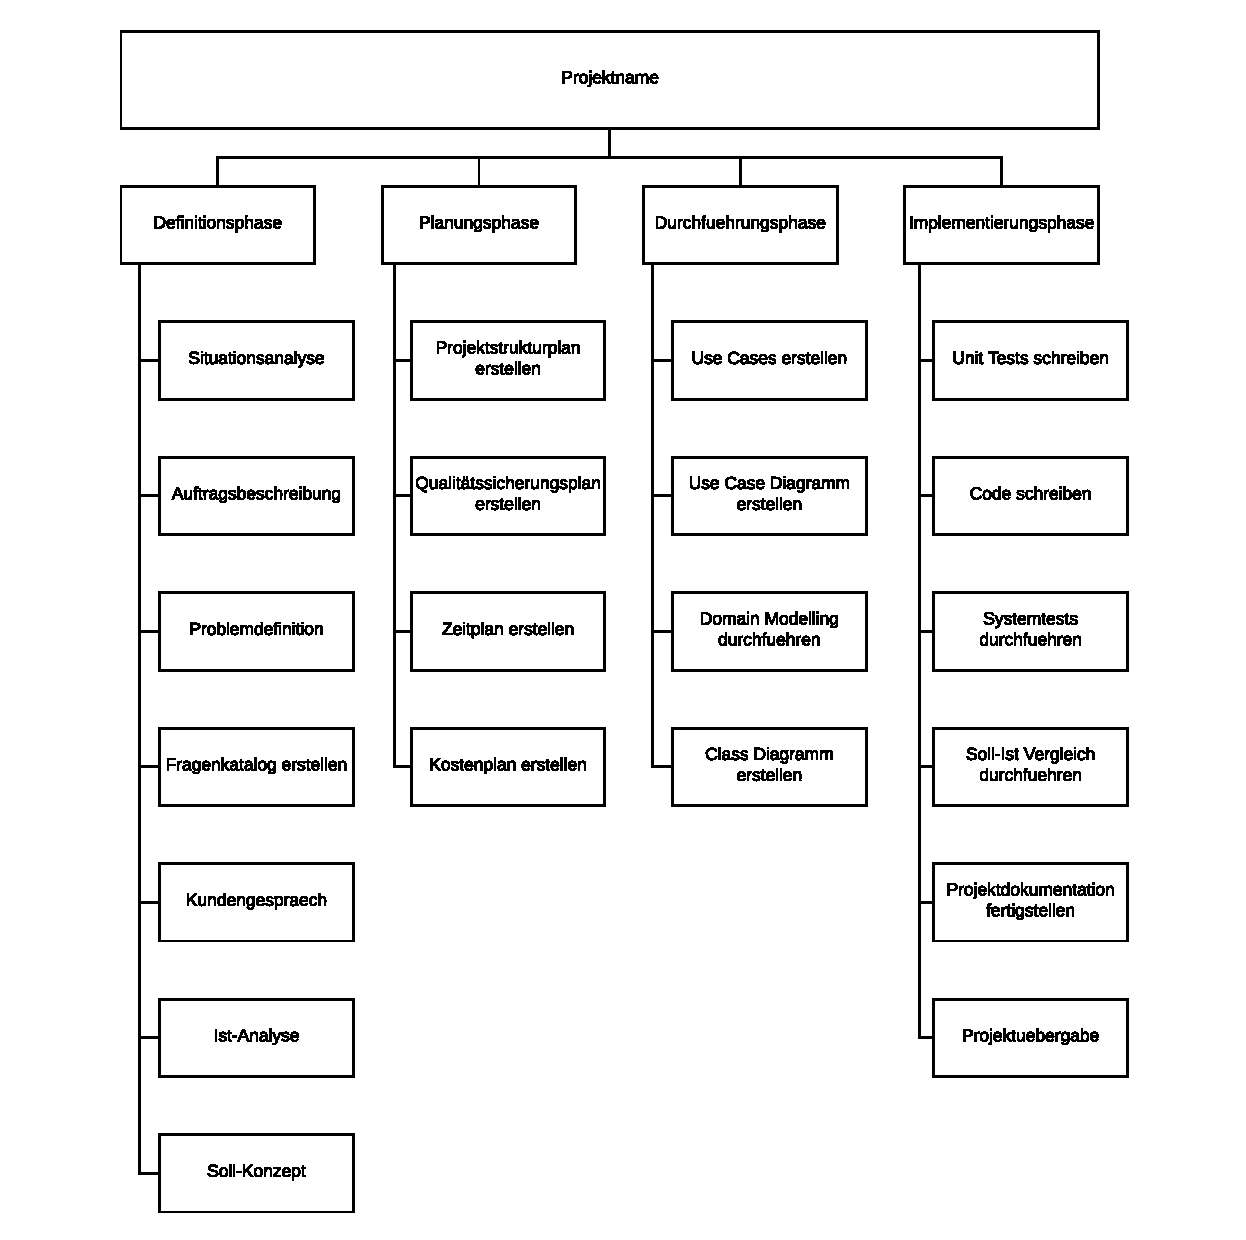
\includegraphics[width=1.4\linewidth]{fig/Projektstrukturplan.pdf}}
  \caption{Projektstrukturplan}
  \label{fig:psp}
\end{figure}
\newpage

% Terminplan Table
\begin{table}[h!]
  \begin{center}
    \caption{Zeitplan}
    \label{table1}
    \pgfplotstabletypeset[
      multicolumn names, % allows to have multicolumn names
      col sep=comma, % the seperator in our .csv file
      header=has colnames,
      columns={Fragen,Antworten},
      columns/Fragen/.style={column type={c|},string type},
      columns/Antworten/.style={column type={c|},string type},
      every head row/.style={
        before row={\toprule}, % have a rule at top
        after row={\midrule}
      },
      every last row/.style={
        after row=\bottomrule % rule at bottom
      }
    ]{csv/zeitplan.csv} % filename/path to file
  \end{center}
\end{table}


\end{document}
